\section{Results}
\label{sec:ep_results}

We present the results of running EP for the four data sets described in Section \ref{sec:ep_application}.

% SIMULATED LINEAR REGRESSION
\subsection{Simulated hierarchical linear regression}
\label{subsec:ep_results_linear}

\begin{figure}
\centering
   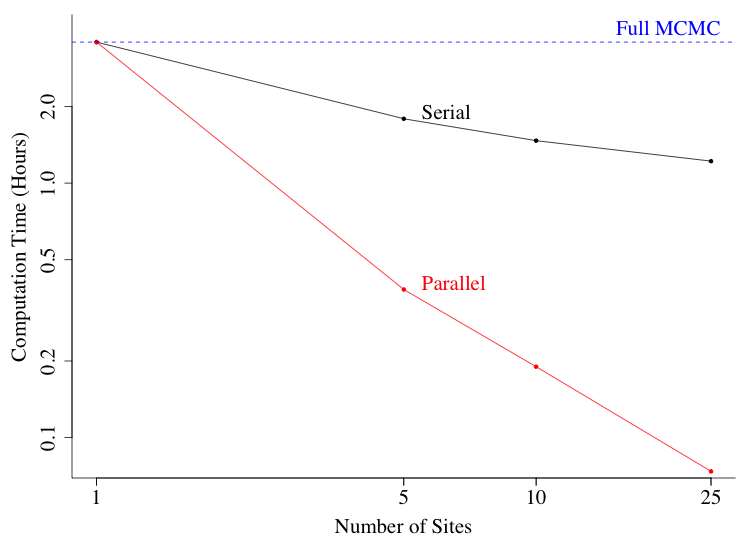
\includegraphics[width=0.65\textwidth]{figures/ep_sim/linear_times.png}
\caption{Computation times for the distributed EP algorithm applied to the simulated linear data set, as a function of the number of sites. The full MCMC computation time is equivalent to that of EP with $K=1$ site.}\label{fig:ep_times_linear}
\end{figure}

Figure~\ref{fig:ep_times_linear} illustrates the computation times for the EP runs with both serial and parallel updates, applied to data simulated from the hierarchical linear model. Because the model is quite simple, serial EP alone gives serious computational advantages. With K = 10 sites, for example, EP provides a 59\% decrease in computation time. The advantages of distributed EP are clear as well, with K = 10 sites resulting in an overall 95\% decrease in computation time. Splitting the computation across K = 25 sites, however, does not provide much additional computational advantages.

\begin{figure}
\centering
    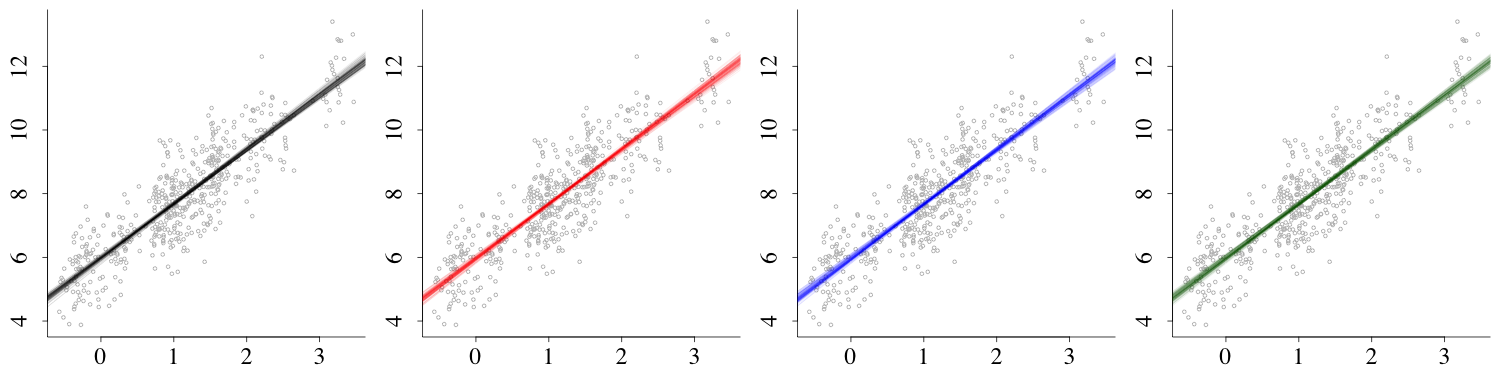
\includegraphics[width=0.8\textwidth]{figures/ep_sim/linear_fit_1.png}
     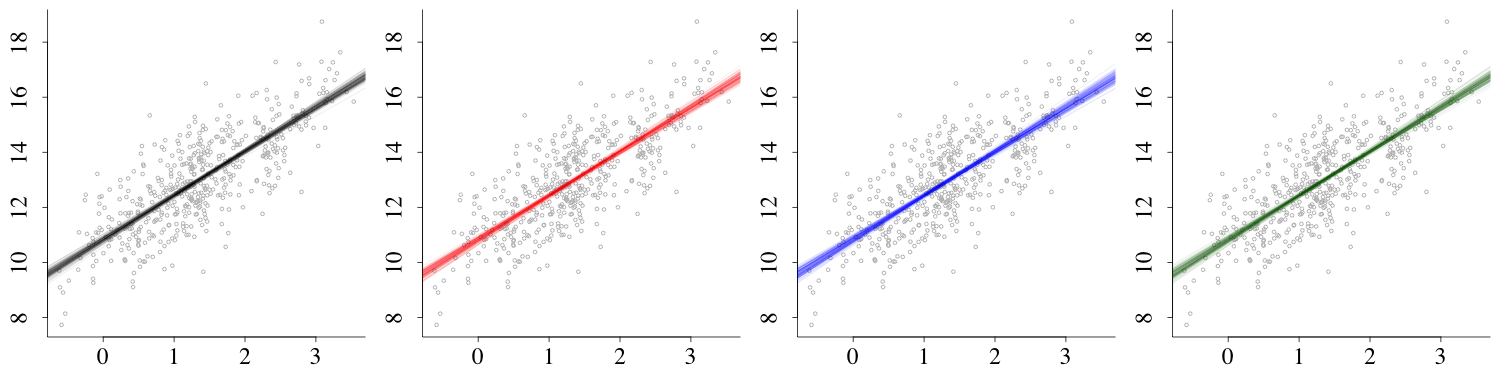
\includegraphics[width=0.8\textwidth]{figures/ep_sim/linear_fit_2.png}
     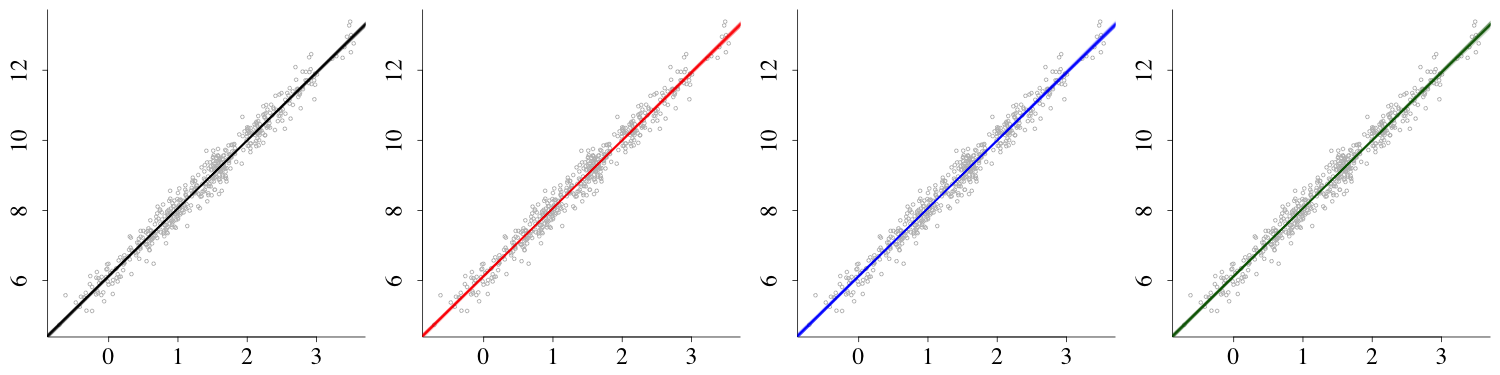
\includegraphics[width=0.8\textwidth]{figures/ep_sim/linear_fit_3.png}
     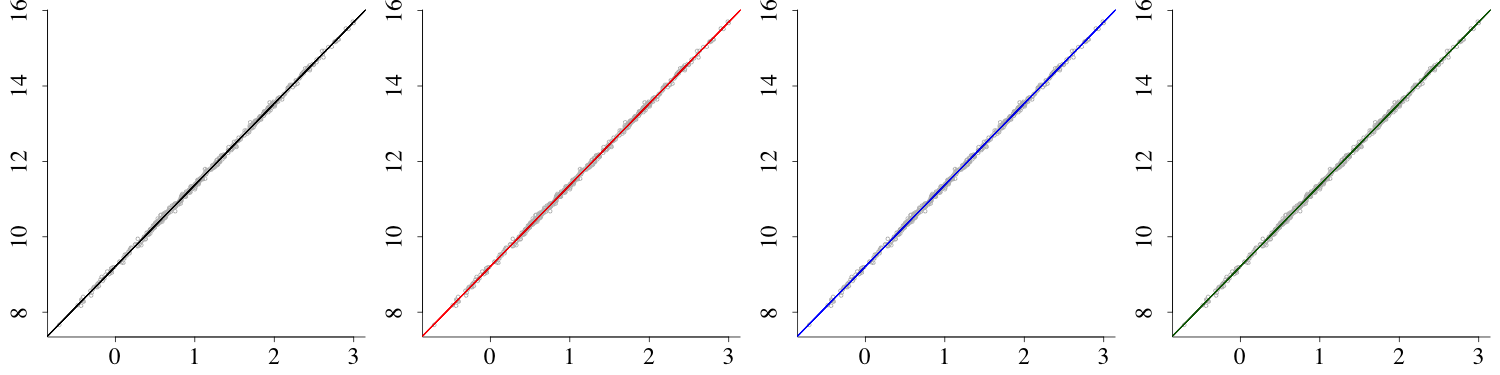
\includegraphics[width=0.8\textwidth]{figures/ep_sim/linear_fit_4.png}
     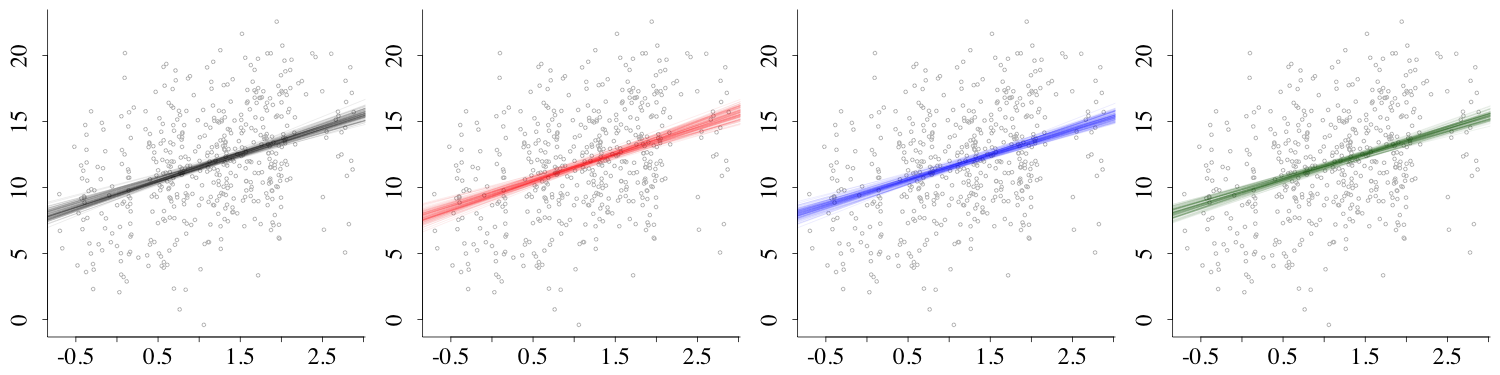
\includegraphics[width=0.8\textwidth]{figures/ep_sim/linear_fit_5.png}
\caption{Comparison of the local fits of the full MCMC computation (black) for the hierarchical linear model and the final distributed EP approximations when the groups are distributed into $K=5$ (red), $K=10$ (blue), and $K=30$ (green) sites. Posterior draws are shown for each of 5 groups (one group per row) with $j = 19, 22, 26, 45,$ and $47$.}
\label{fig:ep_results_linear}
\end{figure}

Figure~\ref{fig:ep_results_linear} shows a comparison of the local scatterplot fits for each EP setting on various hierarchical groups. All of the runs show similar results for all groups, which is somewhat expected for a model this simple. 

% SIMULATED SIGMOID
\subsection{Simulated hierarchical logistic regression}
\label{subsec:ep_results_logistic}

\begin{figure}
\centering
   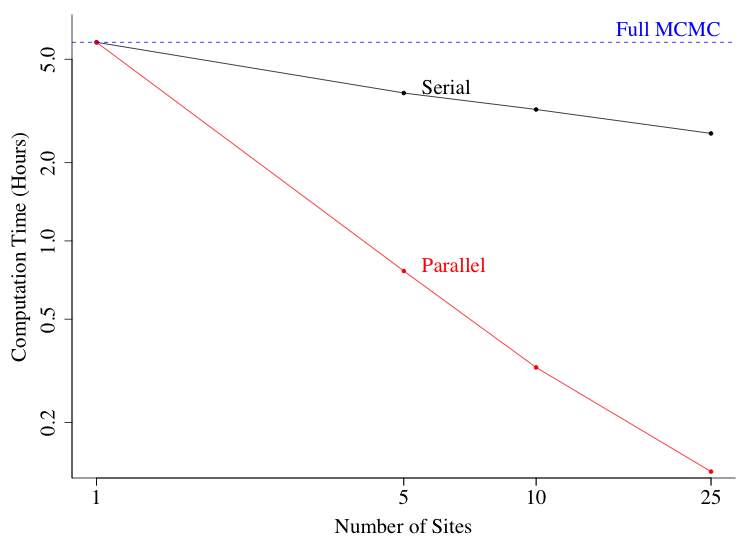
\includegraphics[width=0.65\textwidth]{figures/ep_sim/sigmoid_times.png}
\caption{Computation times for the distributed EP algorithm applied to the simulated sigmoid data set, as a function of the number of sites. The full MCMC computation time is equivalent to that of EP with $K=1$ site.}\label{fig:ep_times_sigmoid}
\end{figure}

Figure~\ref{fig:ep_times_sigmoid} illustrates the computation times for the EP runs with both serial and parallel updates, applied to data simulated from the hierarchical sigmoid model. Compared to the linear model results in Figure \ref{fig:ep_times_linear}, serial EP doesn't provide as large computation advantages. With K = 10 sites, for example, EP provides a 45\% decrease in computation time. The advantages of distributed EP, however, are as pronounced, with K = 10 sites creating an overall 94\% decrease in computation time over the full MCMC approach. Once again, splitting the computation across K = 25 sites does not provide much additional computational advantages.

\begin{figure}
\centering
    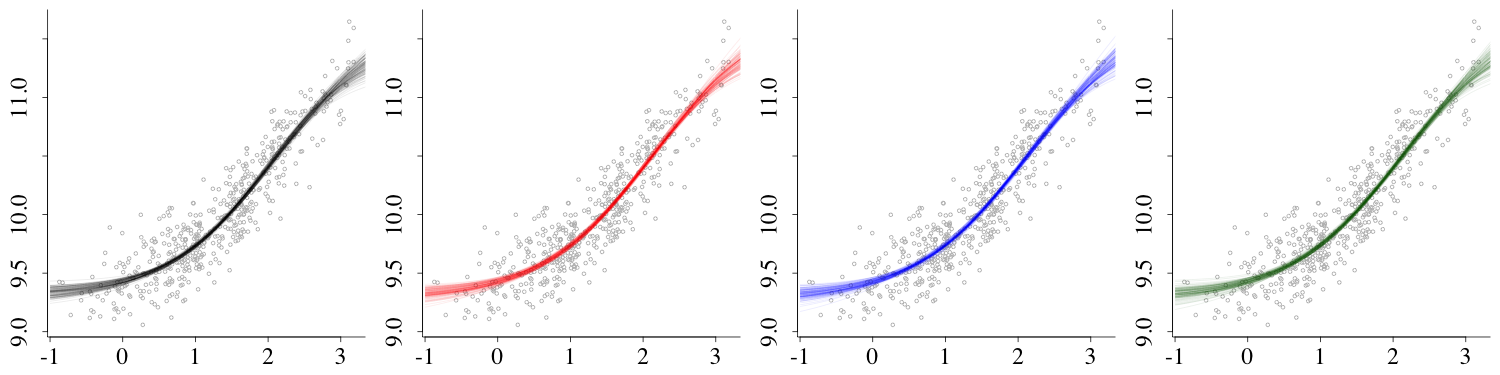
\includegraphics[width=0.8\textwidth]{figures/ep_sim/sigmoid_fit_1.png}
     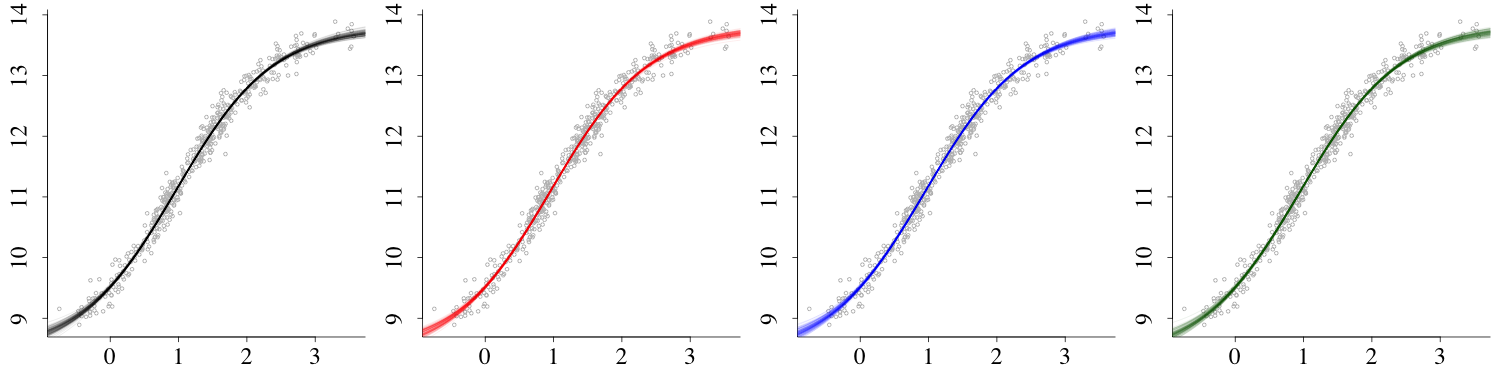
\includegraphics[width=0.8\textwidth]{figures/ep_sim/sigmoid_fit_2.png}
     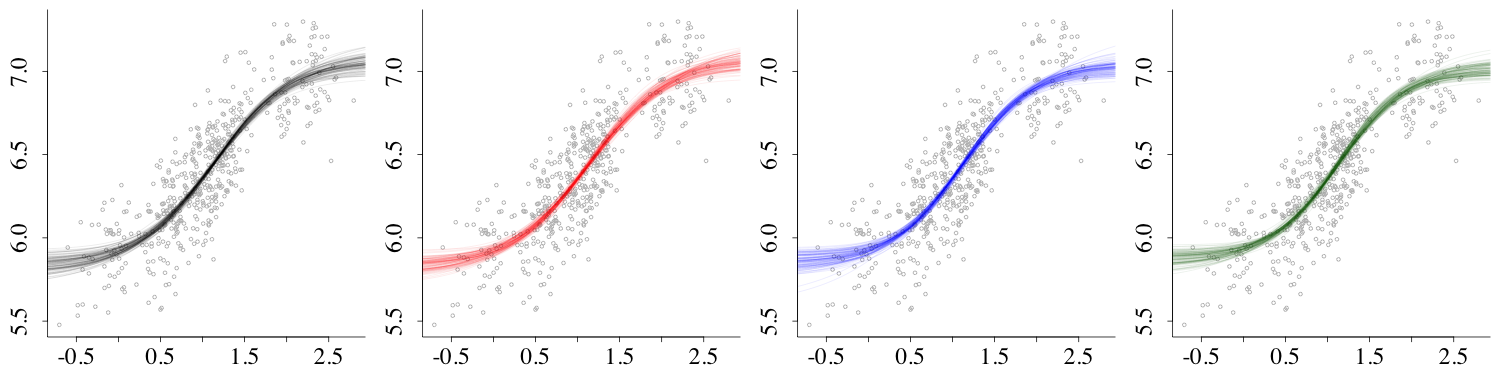
\includegraphics[width=0.8\textwidth]{figures/ep_sim/sigmoid_fit_3.png}
     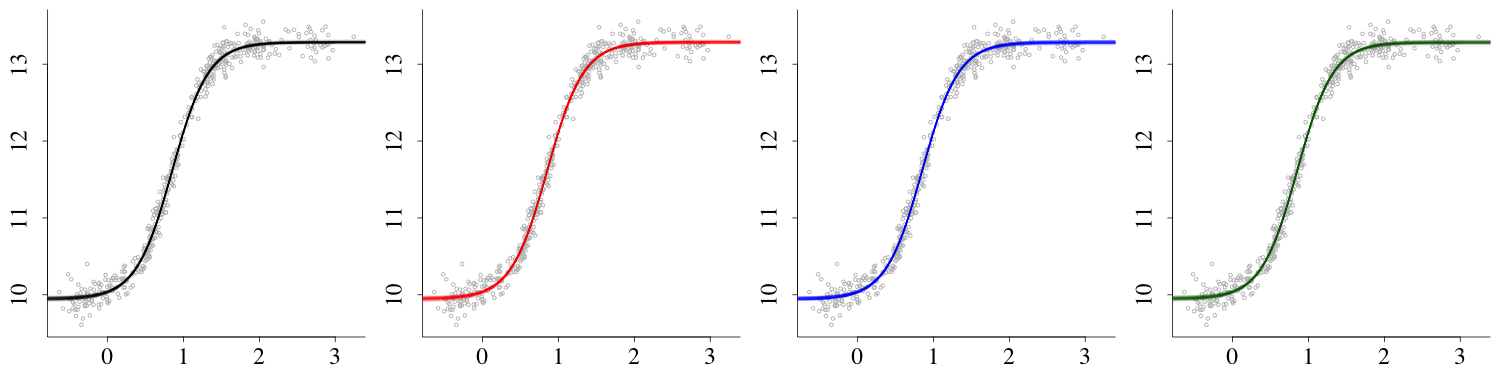
\includegraphics[width=0.8\textwidth]{figures/ep_sim/sigmoid_fit_4.png}
     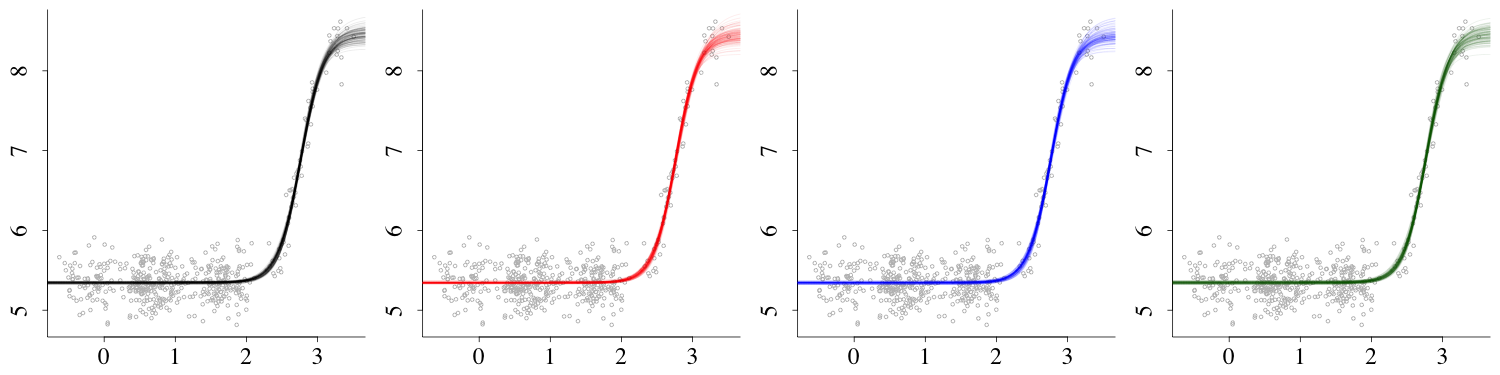
\includegraphics[width=0.8\textwidth]{figures/ep_sim/sigmoid_fit_5.png}
\caption{Comparison of the local fits of the full MCMC computation (black) for the hierarchical sigmoid model and the final distributed EP approximations when the groups are distributed into $K=5$ (red), $K=10$ (blue), and $K=30$ (green) sites. Posterior draws are shown for each of 5 groups (one group per row) with $j = 25, 27, 42, 48,$ and $49$.}
\label{fig:ep_results_sigmoid}
\end{figure}

Figure~\ref{fig:ep_results_sigmoid} shows a comparison of the local scatterplot fits for each EP setting on various hierarchical groups. As with the linear model in Figure \ref{fig:ep_results_linear}, all of the runs show similar results across all groups, which is expected for a model this simple. Models involving more nonlinearities, however, would be expected to take some performance hits as the number of sites is increased.

% SIMULATED SIGMOID WITH DIP
\subsection{Simulated hierarchical logistic regression with dip}
\label{subsec:ep_results_logistic_dip}

\begin{figure}
\centering
   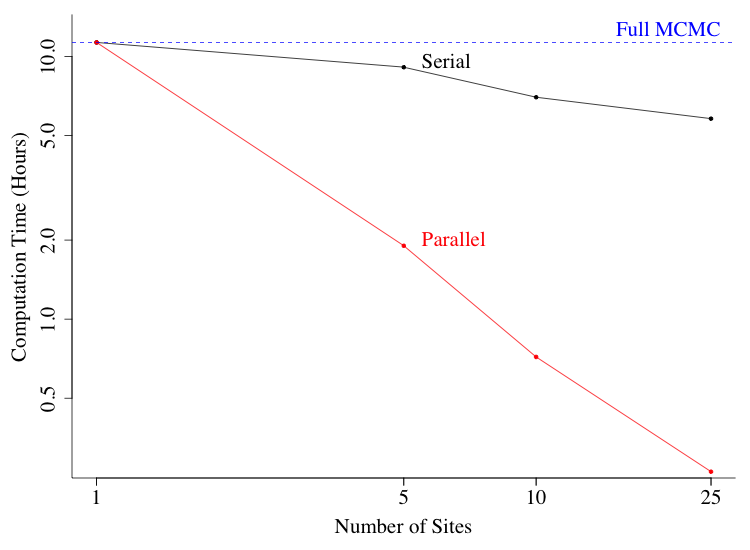
\includegraphics[width=0.65\textwidth]{figures/ep_sim/sigmoid_dip_times.png}
\caption{Computation times for the distributed EP algorithm applied to the simulated sigmoid with dip data set, as a function of the number of sites. The full MCMC computation time is equivalent to that of EP with $K=1$ site.}\label{fig:ep_times_sigmoid_dip}
\end{figure}

Figure~\ref{fig:ep_times_sigmoid_dip} illustrates the computation times for the EP runs with both serial and parallel updates, applied to data simulated from the hierarchical sigmoid with dip model. Compared to the linear and sigmoid model results in Figures \ref{fig:ep_times_linear} and \ref{fig:ep_times_sigmoid}, serial EP provides even fewer computation advantages. With K = 10 sites, EP provides only a 38\% decrease in computation time. The advantages of distributed EP, however, are just as pronounced, with K = 10 sites creating an overall 94\% decrease in computation time over the full MCMC approach. Once again, splitting the computation across K = 25 sites does not provide much additional computational advantages.

\begin{figure}
\centering
    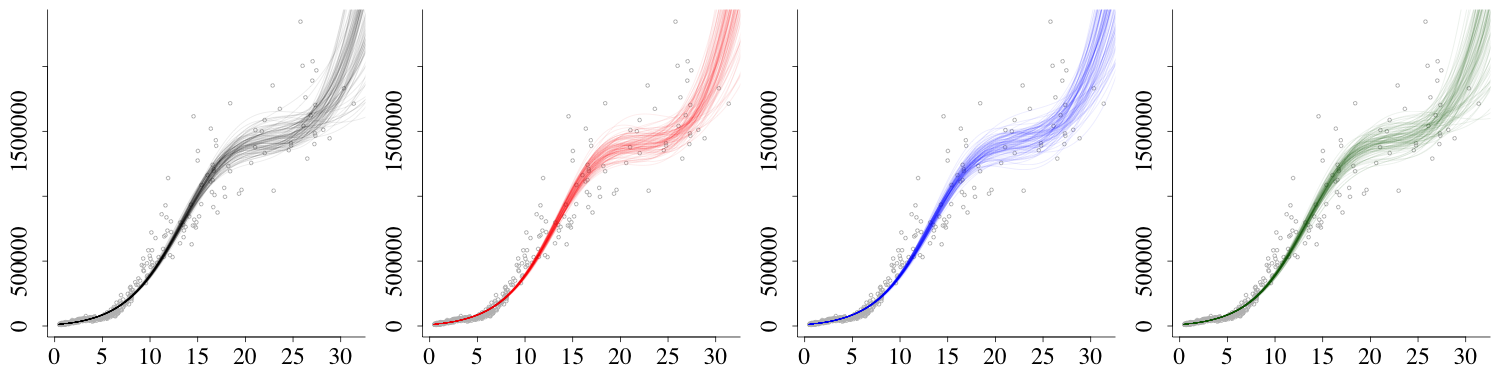
\includegraphics[width=0.8\textwidth]{figures/ep_sim/sigmoid_dip_fit_1.png}
     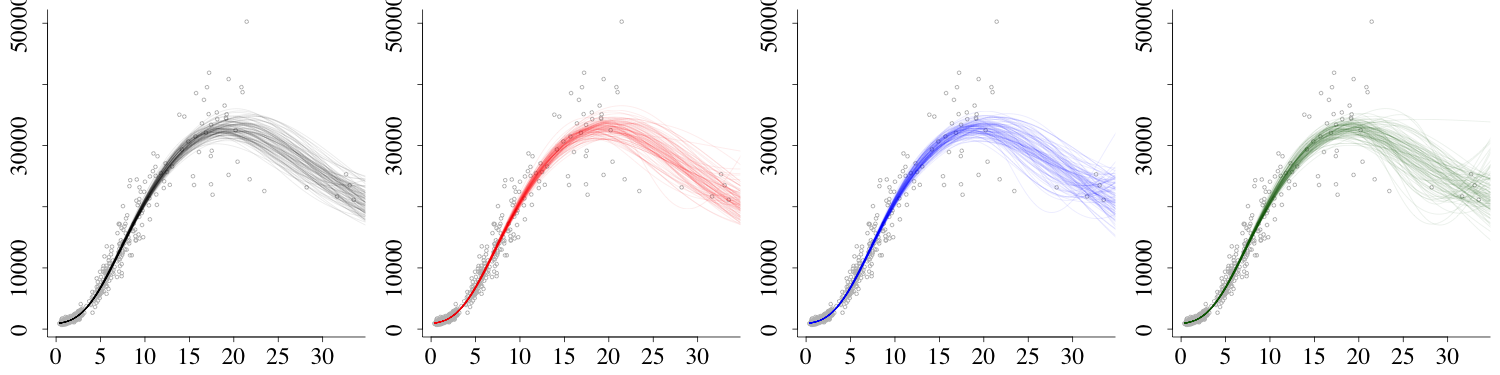
\includegraphics[width=0.8\textwidth]{figures/ep_sim/sigmoid_dip_fit_2.png}
     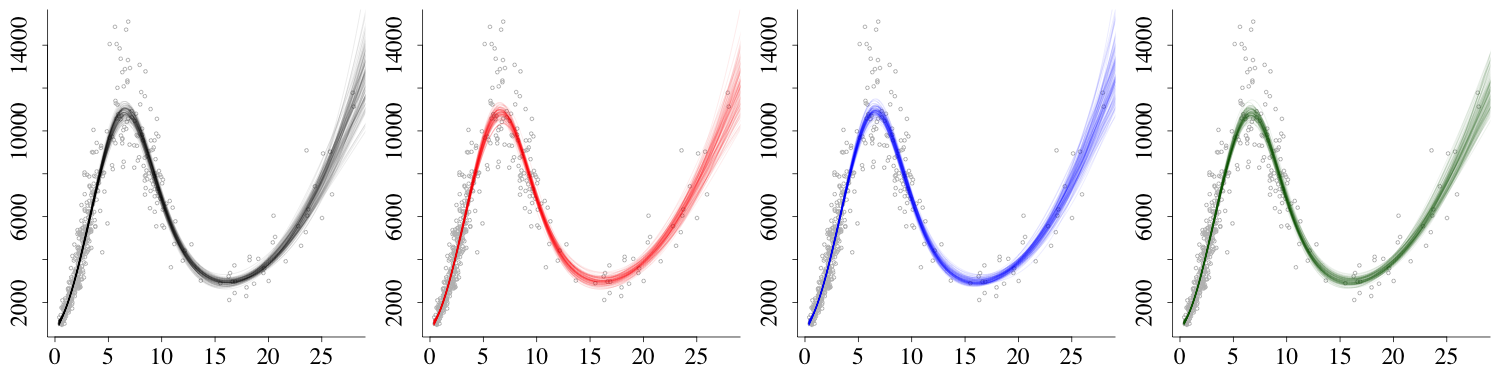
\includegraphics[width=0.8\textwidth]{figures/ep_sim/sigmoid_dip_fit_3.png}
     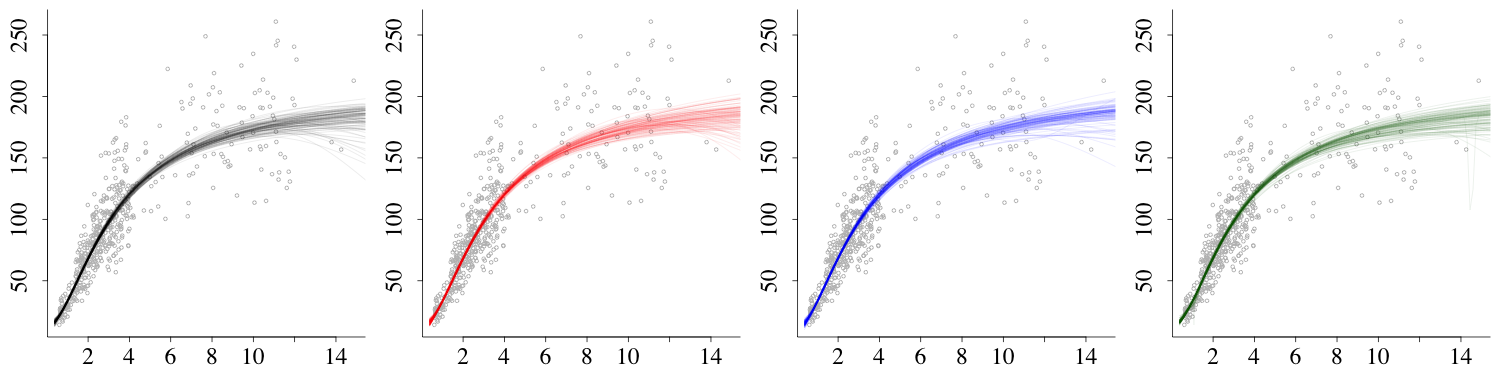
\includegraphics[width=0.8\textwidth]{figures/ep_sim/sigmoid_dip_fit_4.png}
     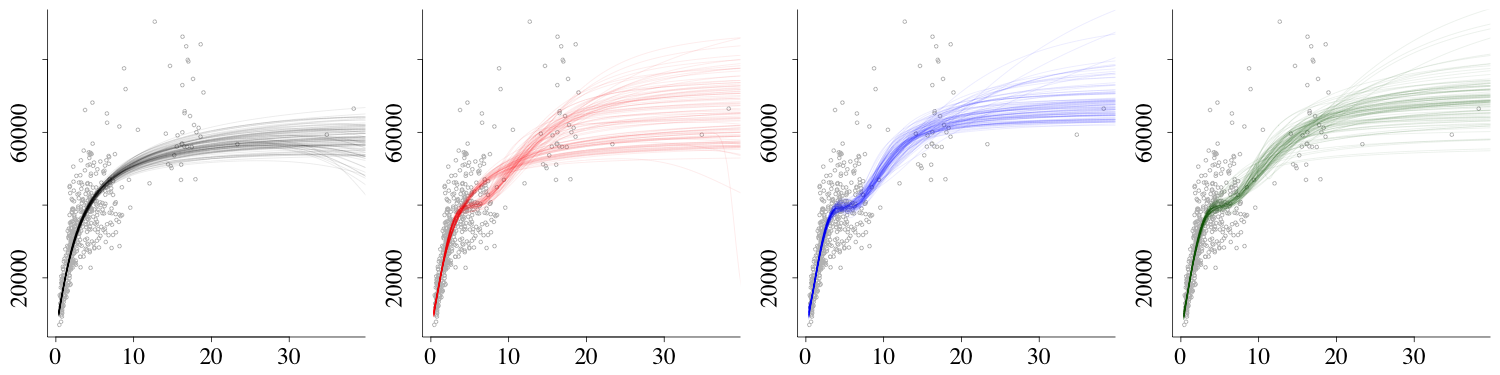
\includegraphics[width=0.8\textwidth]{figures/ep_sim/sigmoid_dip_fit_5.png}
\caption{Comparison of the local fits of the full MCMC computation (black) for the hierarchical sigmoid with dip model and the final distributed EP approximations when the groups are distributed into $K=5$ (red), $K=10$ (blue), and $K=30$ (green) sites. Posterior draws are shown for each of 5 groups (one group per row) with $j = 1, 3, 33, 42,$ and $48$.}
\label{fig:ep_results_sigmoid_dip}
\end{figure}

Figure~\ref{fig:ep_results_sigmoid_dip} shows a comparison of the local scatterplot fits for each EP setting on various hierarchical groups. While most of the runs show similar results across all groups, this is the first model were we begin to see some of the limitations of distributed EP. Namely, for group 48 (the fifth column), the run with $K = 5$ sites arrives at a different posterior distribution over the local parameters compared to the full MCMC run. This limitation is something we would expect to see every so often for more complex nonlinear models such as the one experimented with here.

% ASTRONOMY DATA
\subsection{Galactic ultraviolet data}
\label{subsec:ep_results_astro}

\begin{figure}
\centering
   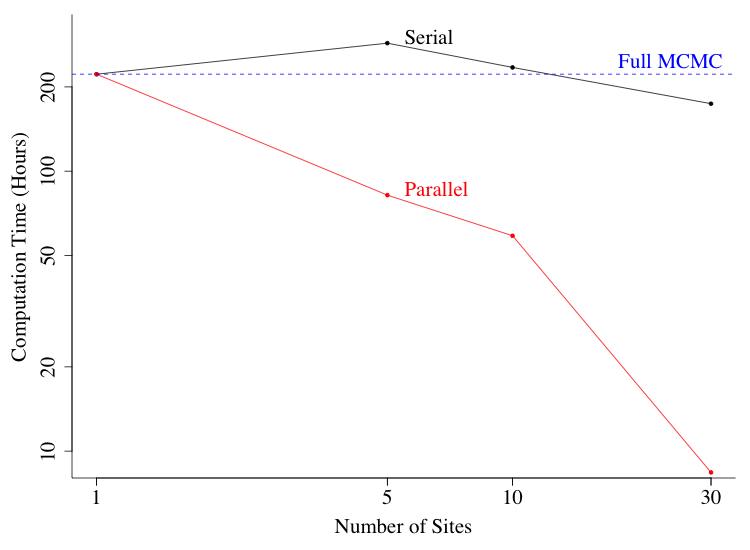
\includegraphics[width=0.65\textwidth]{figures/astro_times}
\caption{Computation times for the distributed EP algorithm applied to the astronomy data set, as a function of the number of sites. The full MCMC computation time is equivalent to that of EP with $K=1$ site.}\label{fig:astro_times}
\end{figure}

Figure~\ref{fig:astro_times} illustrates the computation times for the EP runs with both serial and parallel updates, applied to the real astronomy data. Unlike the simulated data results in Figures \ref{fig:ep_times_linear}, \ref{fig:ep_times_sigmoid}, and \ref{fig:ep_times_sigmoid_dip}, the hierarchical mixture model is so complex that the serial EP computation is slower than the full MCMC computation for K = 5 and 10 sites. As such, the advantages of distributed EP are more important, as seen by K = 10 sites resulting in a 74\% decrease in computation time over full MCMC. This advantage in computation time, however, depends on the implementation of the parallelization. By using the time spent on the sampling of the tilted distribution as our benchmarking criterion, we can focus on the crucial part of the algorithm and neglect the implementation-specific factor.

\begin{figure}
\centering
   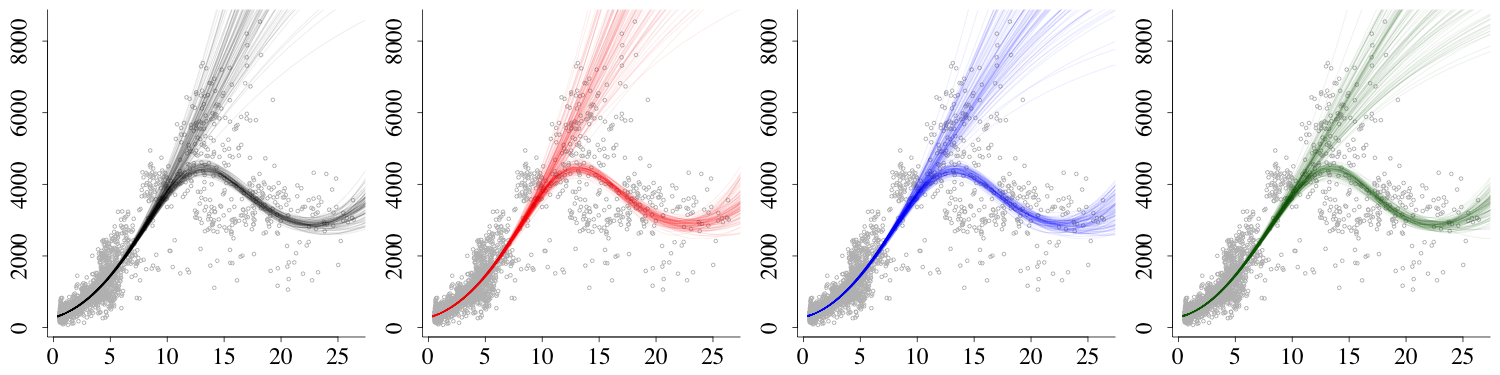
\includegraphics[width=0.8\textwidth]{figures/astro_fit/1}
   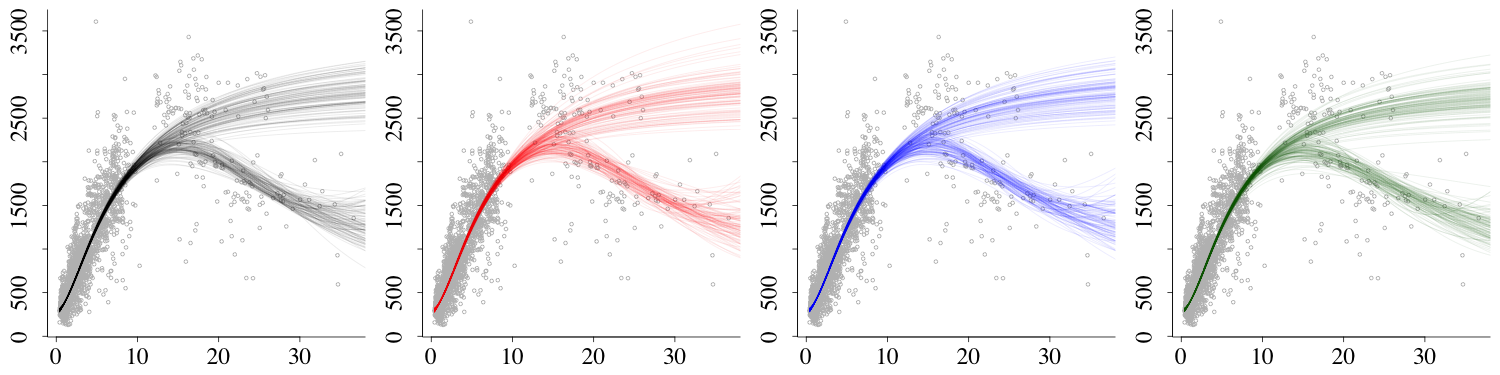
\includegraphics[width=0.8\textwidth]{figures/astro_fit/2}
   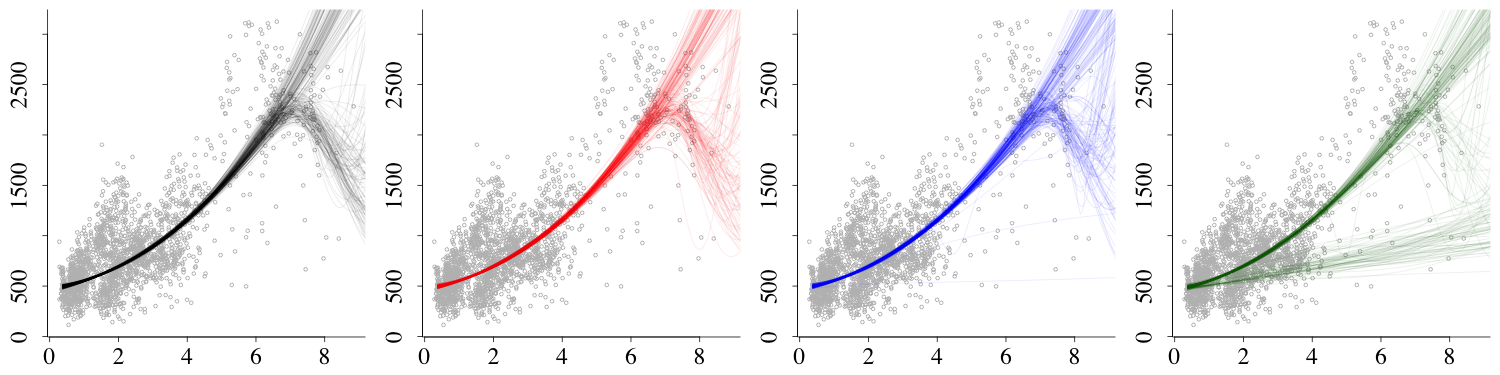
\includegraphics[width=0.8\textwidth]{figures/astro_fit/3}
   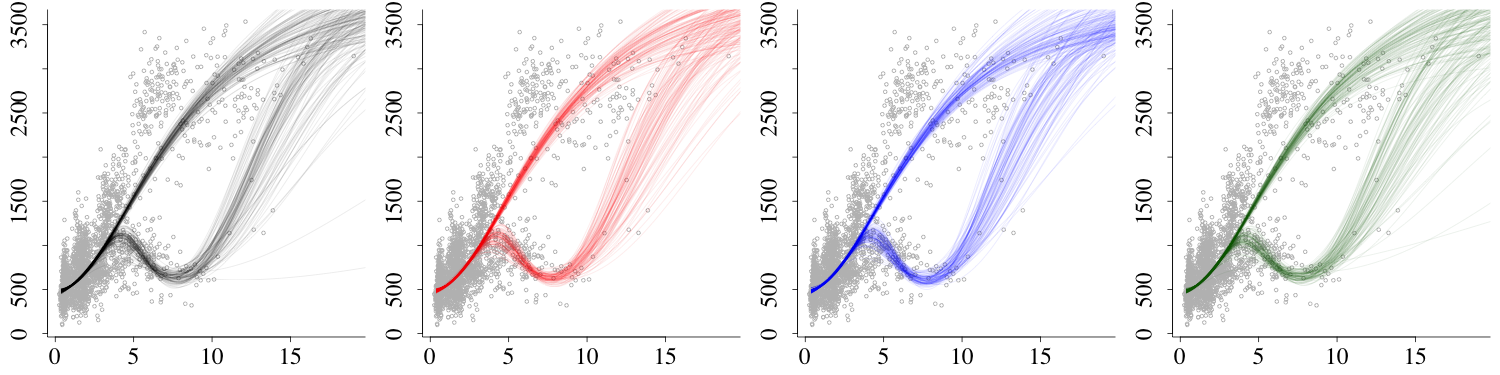
\includegraphics[width=0.8\textwidth]{figures/astro_fit/5}
   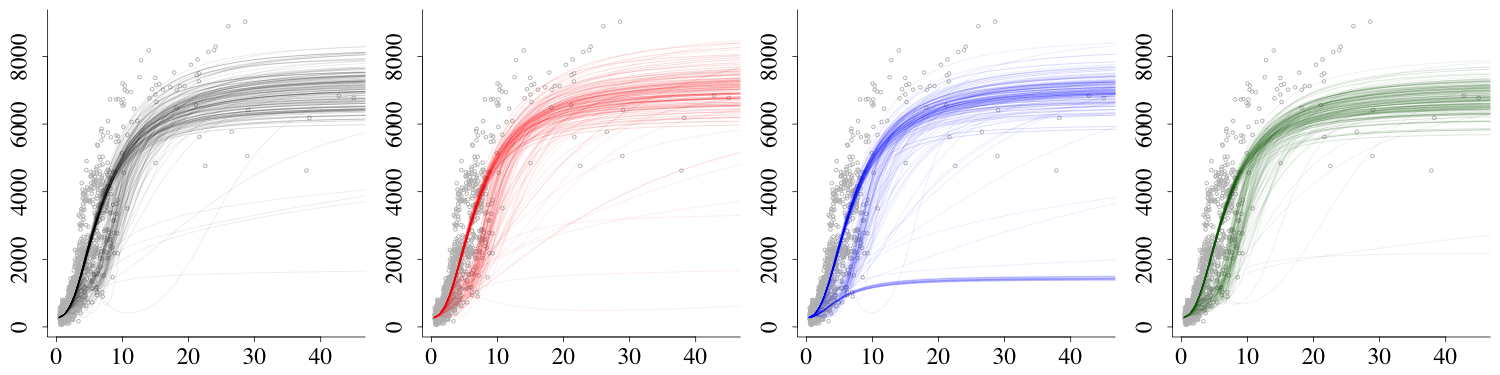
\includegraphics[width=0.8\textwidth]{figures/astro_fit/6}
\caption{Comparison of the local fits of the full MCMC computation (black) for the astronomy example and the final distributed EP approximations when the groups are distributed into $K=5$ (red), $K=10$ (blue), and $K=30$ (green) sites. Posterior draws are shown for longitudes $12\degree, 32\degree, 82\degree, 93\degree,$ and $194\degree$ (one per row).}\label{fig:astro_compare}
\end{figure}

Figure~\ref{fig:astro_compare} shows a comparison of the local scatterplot fits for each EP setting on various hierarchical groups, each representing a one-degree longitudinal slice of the observable universe. While all of the runs show similar results for most groups, there are some cases where increasing the number of sites results in poorer performance. In particular, EP with 30 sites converges to a different mixture for $82\degree$, while EP with 10 sites converges to a different mixture for $194\degree$.